%%%%%%%%%%%%%%%%%%%%%%%%%%%%%%%%%%%%%%%%%%%%%%%%%%%%%%%%%%%%%
%%
%%
%%     NPR's  Nature template...  
%%     v1.0.0   Thu Dec  8 19:05:57 EST 2016
%%                                                                         
%%
%%%%%%%%%%%%%%%%%%%%%%%%%%%%%%%%%%%%%%%%%%%%%%%%%%%%%%%%%%%%%
\documentclass{nature}
%\documentclass{natureprintstyle}

\usepackage{graphicx, fancyhdr, subfigure}
\usepackage{epsfig, psfig, epsf}
\usepackage{amsmath, amssymb, cancel, mathptmx}
\usepackage[T1]{fontenc}
\usepackage{dcolumn}  %%  Align table columns on decimal point
\usepackage{bm}           %%  bold math
\usepackage{hyperref,ifthen}
\usepackage{verbatim, threeparttable}
\usepackage[sort,comma,numbers]{natbib}

\newcommand{\oiii}{[O\,{\sc iii}]\ }
\newcommand{\nii}{N\,{\sc ii}\ }


\bibliographystyle{naturemag}

\title{A new physical interpretation of optical and infrared variability in quasars}

\author{Nicholas~P.~Ross$^{1}$,    
K. E. Saavik Ford$^{2,3,4}$,  
Matthew Graham$^{5}$,  
Barry McKernan$^{2,3,4}$,  
Daniel Stern$^{5,6}$, 
Aaron M. Meisner$^{7,8}$, 
Roberto Assef$^{9}$, 
Arjun Dey$^{10}$,
%George Djorgovsk 
Andrew J. Drake$^{11}$, 
%Peter Eisenhardt, 
Hyunsung D. Jun$^{12}$ 
%David Schlegel, 
}

\begin{document}

\maketitle

\begin{affiliations}
  \item Institute for Astronomy, University of Edinburgh, Royal Observatory, Blackford Hill, Edinburgh EH9 3HJ, United Kingdom 
  \item Department of Science, BMCC, City University of New York, New York, NY 10007, USA
 \item Department of Astrophysics, American Museum of Natural History, Central Park West at 79th Street, NY 10024, USA
 \item  Graduate Center, City University of New York, 365 5th Avenue, New York, NY 10016, USA
\item Cahill Center for Astronomy and Astrophysics, California Institute of Technology, Mail Code 249/17, 1200 E California Blvd, Pasadena CA 91125, USA
% \item Department of Astrophysics is located in the Rose Center for Earth and Space, American Museum of Natural History, Central Park West at 79th Street, New York, NY 10024, U.S.A
  \item Jet Propulsion Laboratory, California Institute of Technology, 4800 Oak Grove Drive, Mail Stop 169-221, Pasadena, CA 91109, USA 
  \item Lawrence Berkeley National Laboratory, 1 Cyclotron Road, Berkeley, CA 92420, U.S.A. 
  \item  Berkeley Center for Cosmological Physics, Berkeley, CA 94720, USA
\item N\'ucleo de Astronom\'ia de la Facultad de Ingenier\'ia,  Universidad Diego Portales, Av. Ej\'ercito Libertador 441, Santiago,
  Chile
  %\item Steward Observatory, 933 North Cherry Avenue, Tucson, AZ 85721, U.S.A.
\item National Optical Astronomy Observatory, 950 N. Cherry Ave, Tucson, AZ 85719, USA
\item Center for Advanced Computing Research, California Institute of Technology, 1200 E California Blvd, Pasadena CA 91125, USA
\item School of Physics, Korea Institute for Advanced Study, 85 Hoegiro, Dongdaemun-gu, Seoul 02455, Korea
%  \item Universidad Diego Portales, Av Republica 180, Santiago, Regi ́on Metropolitana, Chile}
\end{affiliations}


\begin{abstract}
Changing-look quasars are a recently identified class of active
galaxies in which the strong UV continuum and/or broad optical
hydrogen emission lines associated with unobscured quasars either
appear or disappear on timescales of months to years
\cite{LaMassa2015, Runnoe2016, MacLeod2016, Ruan2016, Rumbaugh2017,
Yang2017}.  The physical processes responsible for this behaviour are
still debated, but changes in the black hole accretion rate or
accretion disk structure appear more likely than changes in
obscuration \cite{Hutsemekers2017, Sheng2017}.  Here we report on four
epochs of spectroscopy of SDSS J110057.70-005304.5, a quasar at a
redshift of $z=0.378$ whose UV continuum and broad hydrogen emission
lines have faded, and then returned over the past $\approx$20
years. The change in this quasar was initially identified in the
infrared, and an archival spectrum from 2010 shows an intermediate
phase of the transition during which the flux below rest-frame
3400\AA\ has decreased by close to an order of magnitude. This
combination is unique compared to previously published examples of
changing-look quasars, and is best explained by dramatic changes in
the innermost regions of the accretion disk. The optical continuum has
been rising since mid-2016, leading to a prediction of a rise in
hydrogen emission line flux in the next year. Increases in the
infrared flux should follow, occurring on a $\sim$3 year observed
timescale. If our model is confirmed, the physics of changing-look
quasars are governed by processes at the innermost stable circular
orbit (ISCO) around the black hole, and the structure of the innermost
disk. The easily identifiable and monitored changing-look quasars
would then provide a new probe and laboratory of the nuclear central
engine.
\end{abstract}



%%%%%%%%%%%%%%%%%%%%%%%%%%%%%%%%%%%%%%%%%%%%%%%%%%%%%%%%%%%%%%%%%%%%%%%%%%%%%%%%%
%%%%%%%%%%%%%%%%%%%%%%%%%%%%%%%%%%%%%%%%%%%%%%%%%%%%%%%%%%%%%%%%%%%%%%%%%%%%%%%%%
%%
%%
%%   SECTION 1  SECTION 1  SECTION 1  SECTION 1  SECTION 1  SECTION 1  
%%   SECTION 1  SECTION 1  SECTION 1  SECTION 1  SECTION 1  SECTION 1  
%%   SECTION 1  SECTION 1  SECTION 1  SECTION 1  SECTION 1  SECTION 1  
%%
%%
%%%%%%%%%%%%%%%%%%%%%%%%%%%%%%%%%%%%%%%%%%%%%%%%%%%%%%%%%%%%%%%%%%%%%%%%%%%%%%%%%%
%%%%%%%%%%%%%%%%%%%%%%%%%%%%%%%%%%%%%%%%%%%%%%%%%%%%%%%%%%%%%%%%%%%%%%%%%%%%%%%%%%
%\section{Introduction}

The Shakura-Sunyaev $\alpha-$disk model \cite{SS73} has long been used
to (oversimply \cite{Lawrence2018}) describe the basic properties of
the optically thick, geometrically thin accretion disks expected to
orbit the supermassive black holes at the nuclei of quasars.  This
accretion disk is thought to be the origin of thermal continuum
emission observed in the rest-frame ultraviolet and optical. The
$\alpha-$disk model makes the key assumptions that plasma within the
disk is optically thick and thermal, and emission from the accretion
disk can be treated as a superposition of blackbody annuli. Given the
size scales and temperatures associated with supermassive black holes,
a substantial fraction of the bolometric luminosity should be in the
form of UV photons--the so-called ``Big Blue Bump'' \cite{Shields1978,
Malkan_Sargent1982}. By contrast, the thermal emission seen in the
infrared is believed to originate from more distant molecular dust.
Thus, the IR flux is directly proportional to the emission from
the disk, reprocessed by the dusty reservoir and delayed by the
light-travel time between the two \citep[see ][for
reviews]{Antonucci1993, Perlman2008, Lasota2016}.

For the optically thick, UV emitting disk to accrete onto the black
hole, substantial angular momentum must be lost.  A kinematic
viscosity of the plasma, parametrized by $\alpha$, seems the likely
mechanism that transports angular momentum outward.  This viscosity is
likely due to magnetorotational instability \citep[MRI;
][]{Balbus_Hawley1991} with additional contributions to turbulence
from the effects of objects embedded in the disk e.g.,
\cite{McKernan2014}. However, as e.g., \cite{Koratkar_Blaes1999,
Sirko_Goodman2003} point out, the observed spectral energy
distributions (SEDs) of typical quasars differ markedly from classical
$\alpha$-disk theoretical predictions \citep[][]{SS73, Pringle1981}
with a typical observed quasar SED flat in $\lambda F_{\lambda}$ over
several decades in wavelength \citep{Elvis1994,
Richards2006b}. Furthermore, real AGN disks seem to be cooler
\cite[e.g., ][]{Lawrence2012} and larger \cite[e.g.,][]{Pooley2007,
Morgan2010, Morgan2012, Mosquera2011} than the $\alpha$-disk model
predicts. The $\alpha$-disk is an ad hoc parameterization of disk
viscosity and does not permit predictions of global changes from local
perturbations \cite{King2012}. Nevertheless, in this paper, we utilize
the mathematically simple $\alpha$-disk model as a framework and
departure point for our own disk models. Here, we build on previous
work \citep{Goodman2003, Zimmerman2005, Hameury2009} and introduce a
phenomenological model which does allow changes across the accretion
disk and, crucially, makes predictions which can be observed in the
SED.
 
Changing-look quasars have traditionally been discovered by looking
for large, $| \Delta m | >1$ magnitude changes in the optical light
curves of quasars or galaxies. In contrast, we have taken advantage of
the ongoing mid-infrared Near-Earth Object Wide-Field Infrared Survey
Explorer Reactivation mission \cite[NEOWISE-R; ][]{Mainzer2014,
Meisner2017a, Meisner2017b}, supplemented with the optical Dark Energy
Camera Legacy Survey (DECaLS\footnote{{\tt
legacysurvey.org/decamls/}}) in order to discover new changing-look
quasars.  While previous efforts have used the 1-year baseline of the
WISE mission to identify changing-look quasars
\cite[e.g.,][]{Assef2017}, our investigation is the first to extend
this selection to the infrared using NEOWISE-R mission data. We have
identified a sample of Sloan Digital Sky Survey (SDSS) quasars that
show significant changes in their IR flux over the course of a few
years. Importantly, our IR light curves enable us to set limits on SED
changes due to obscuration.

In this article we present the $z=0.378$ quasar SDSS
J110057.70-005304.5 (hereafter J1100-0053).  J1100-0053 was a known
quasar we identified as interesting due to its IR light curve. We have
spectral observations for J1100-0053 showing a transition in the
blue-continuum into a `dim state' where the rest-frame UV flux is
suppressed, and then returning to a blue-continuum sloped quasar.  The
model we present invokes changes at the ISCO to be the triggering
event for substantial changes in the wider accretion disk, including
major structural changes out to 150$r_{g}$ (where $r_{\rm g}$ is the
gravitational radius; $r_{\rm g}=\frac{GM}{c^2}$).  Such a model
explains changes in the broad emission lines, as well as the optical
and IR light curves. 


\begin{figure}
  \centering
  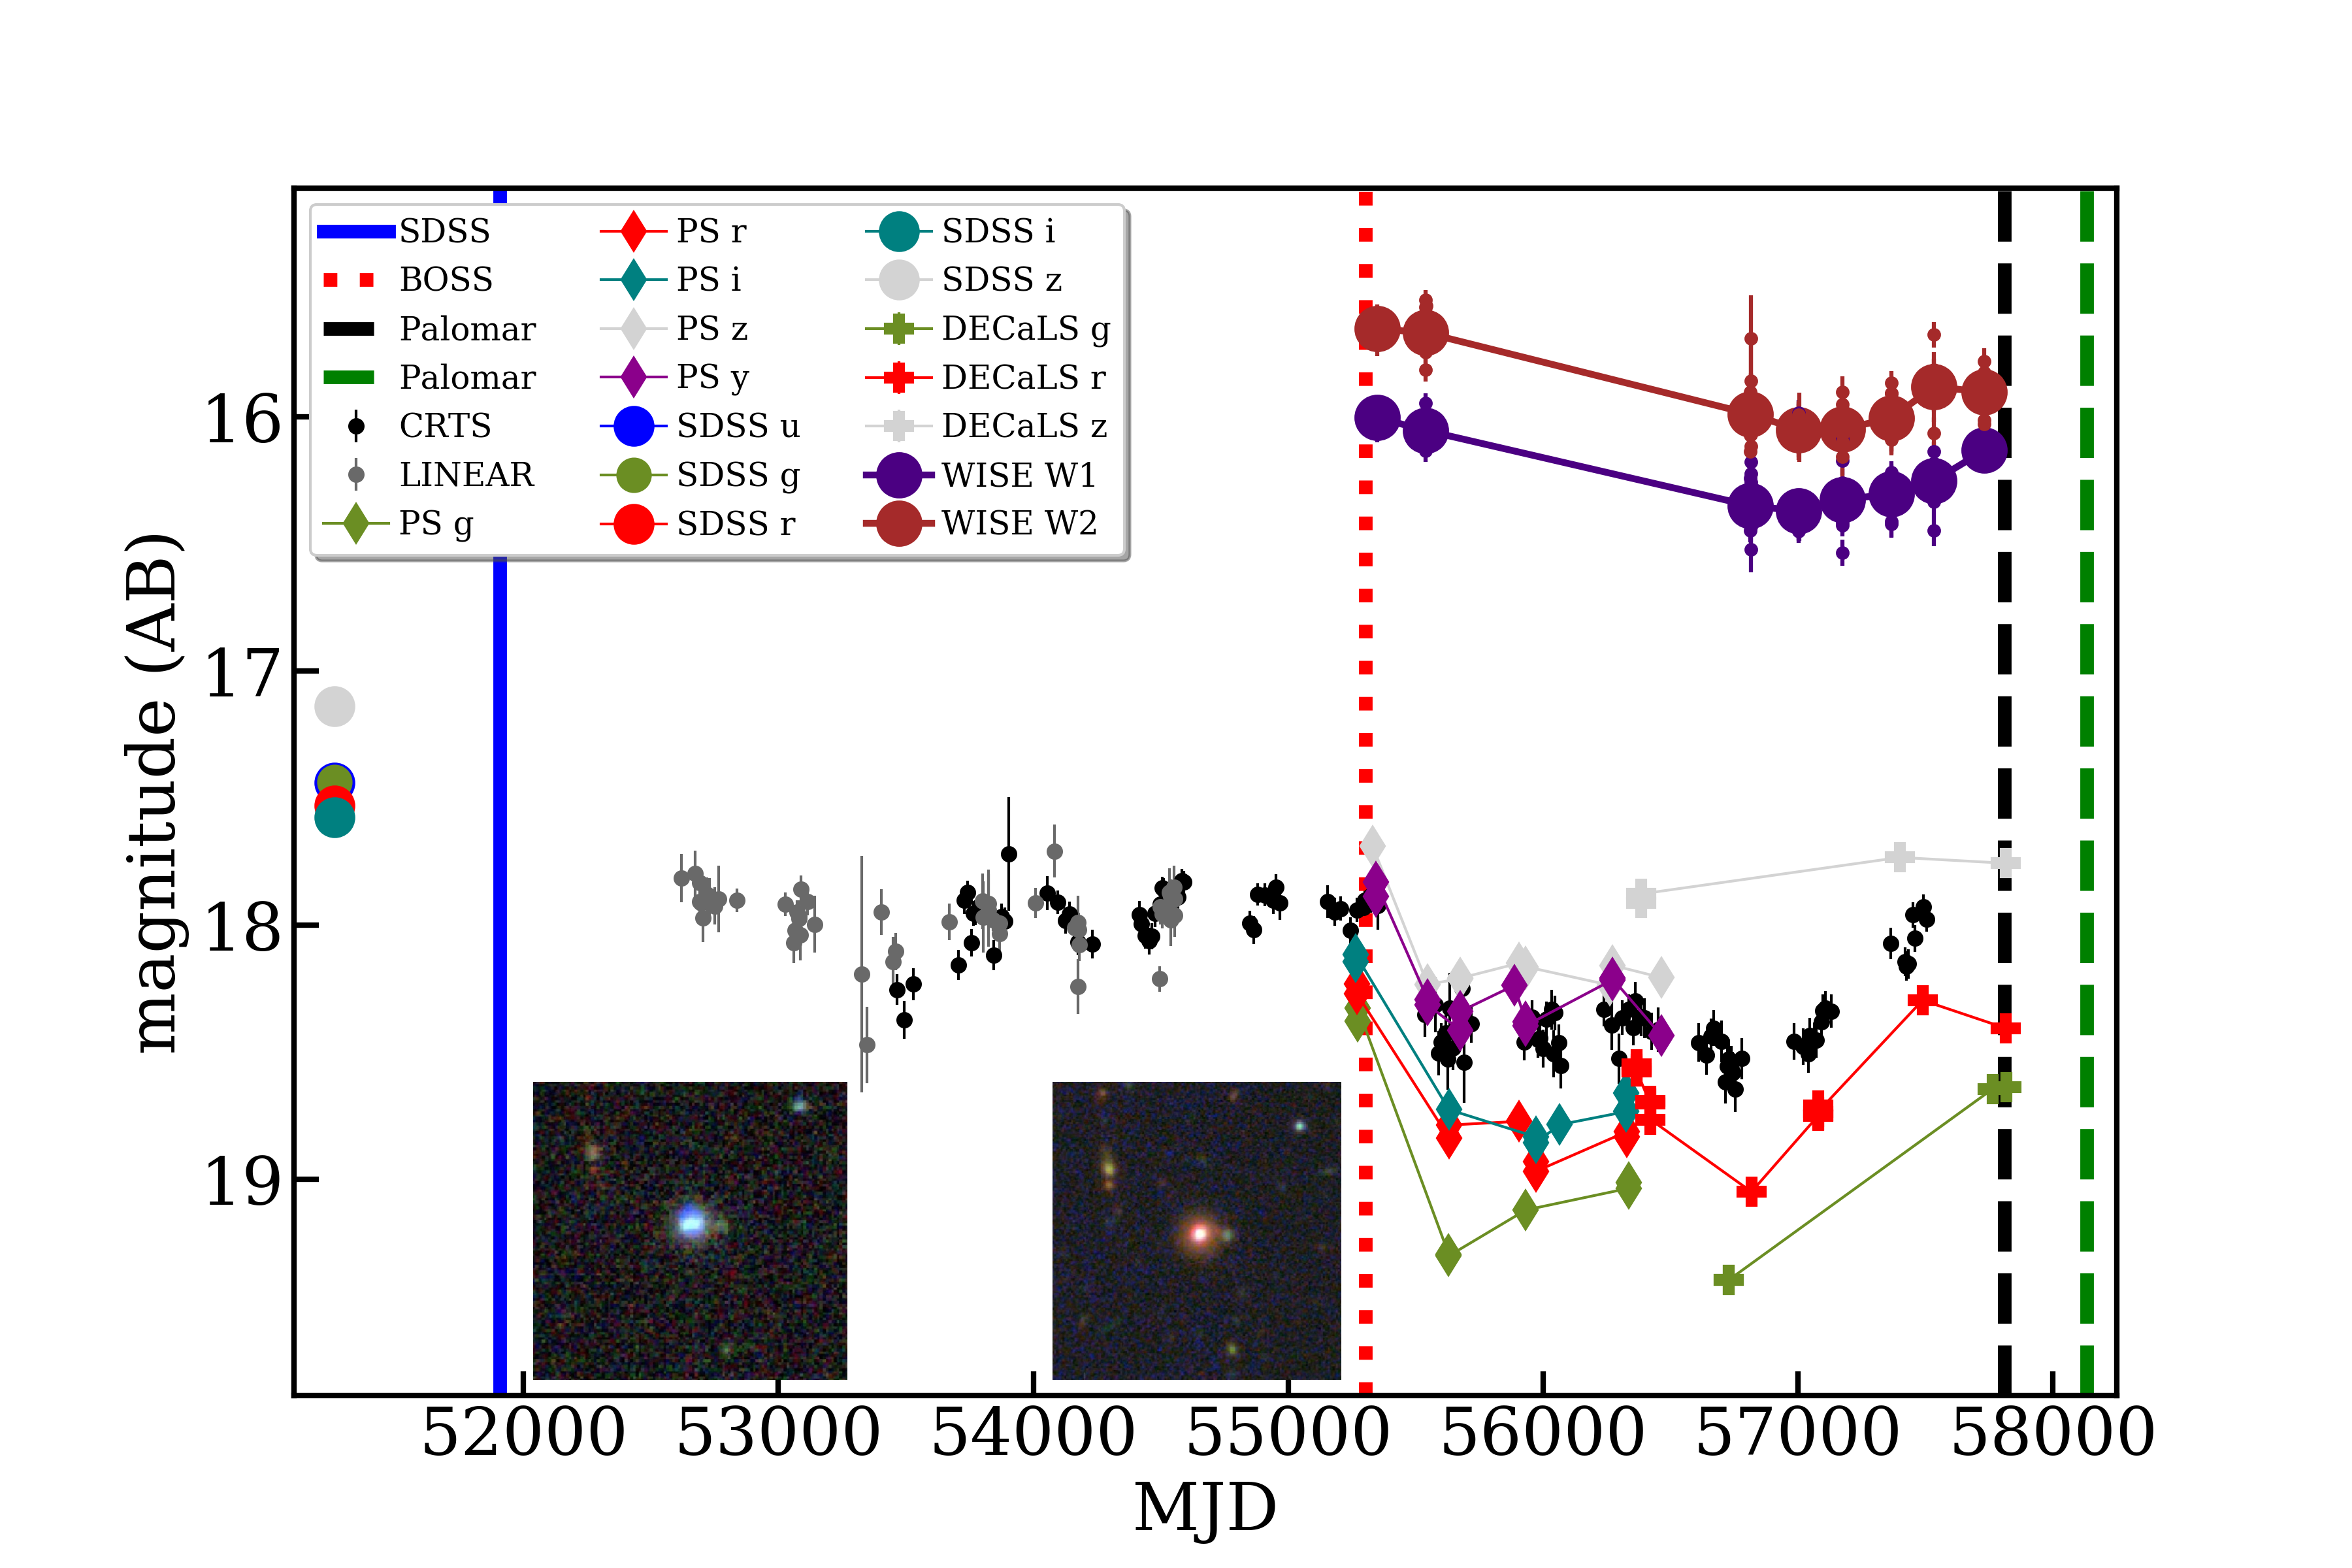
\includegraphics[width=16.00cm, height=10.00cm, trim=0.0cm 0.0cm 0.0cm 0.0cm, clip]
  {../plots/lc/J110057_lc_20180222v1.png}
  \caption[]{
    Multi-wavelength light curve of J1100-0053, including optical data
    from LINEAR, CRTS, SDSS, PanSTARRS and DECaLS, and mid-IR data from
    the WISE satellite.  The four vertical lines illustrate the four
    epochs of optical spectra presented in Figure 2.  J1100-0053 was
    flagged for further study due to the IR fading observed by WISE.  Note
    that the optical emission has been recovering over the past few years,
    with the IR emission beginning to show similar behvaiour. The inserts
    show the images of J1100-0053 from SDSS in 1999 March and the DECaLS DR3
    in 2014 March (50'' on a side). }
  \label{fig:J110057_LC_CRTS}
\end{figure}


\begin{figure}
  \centering
  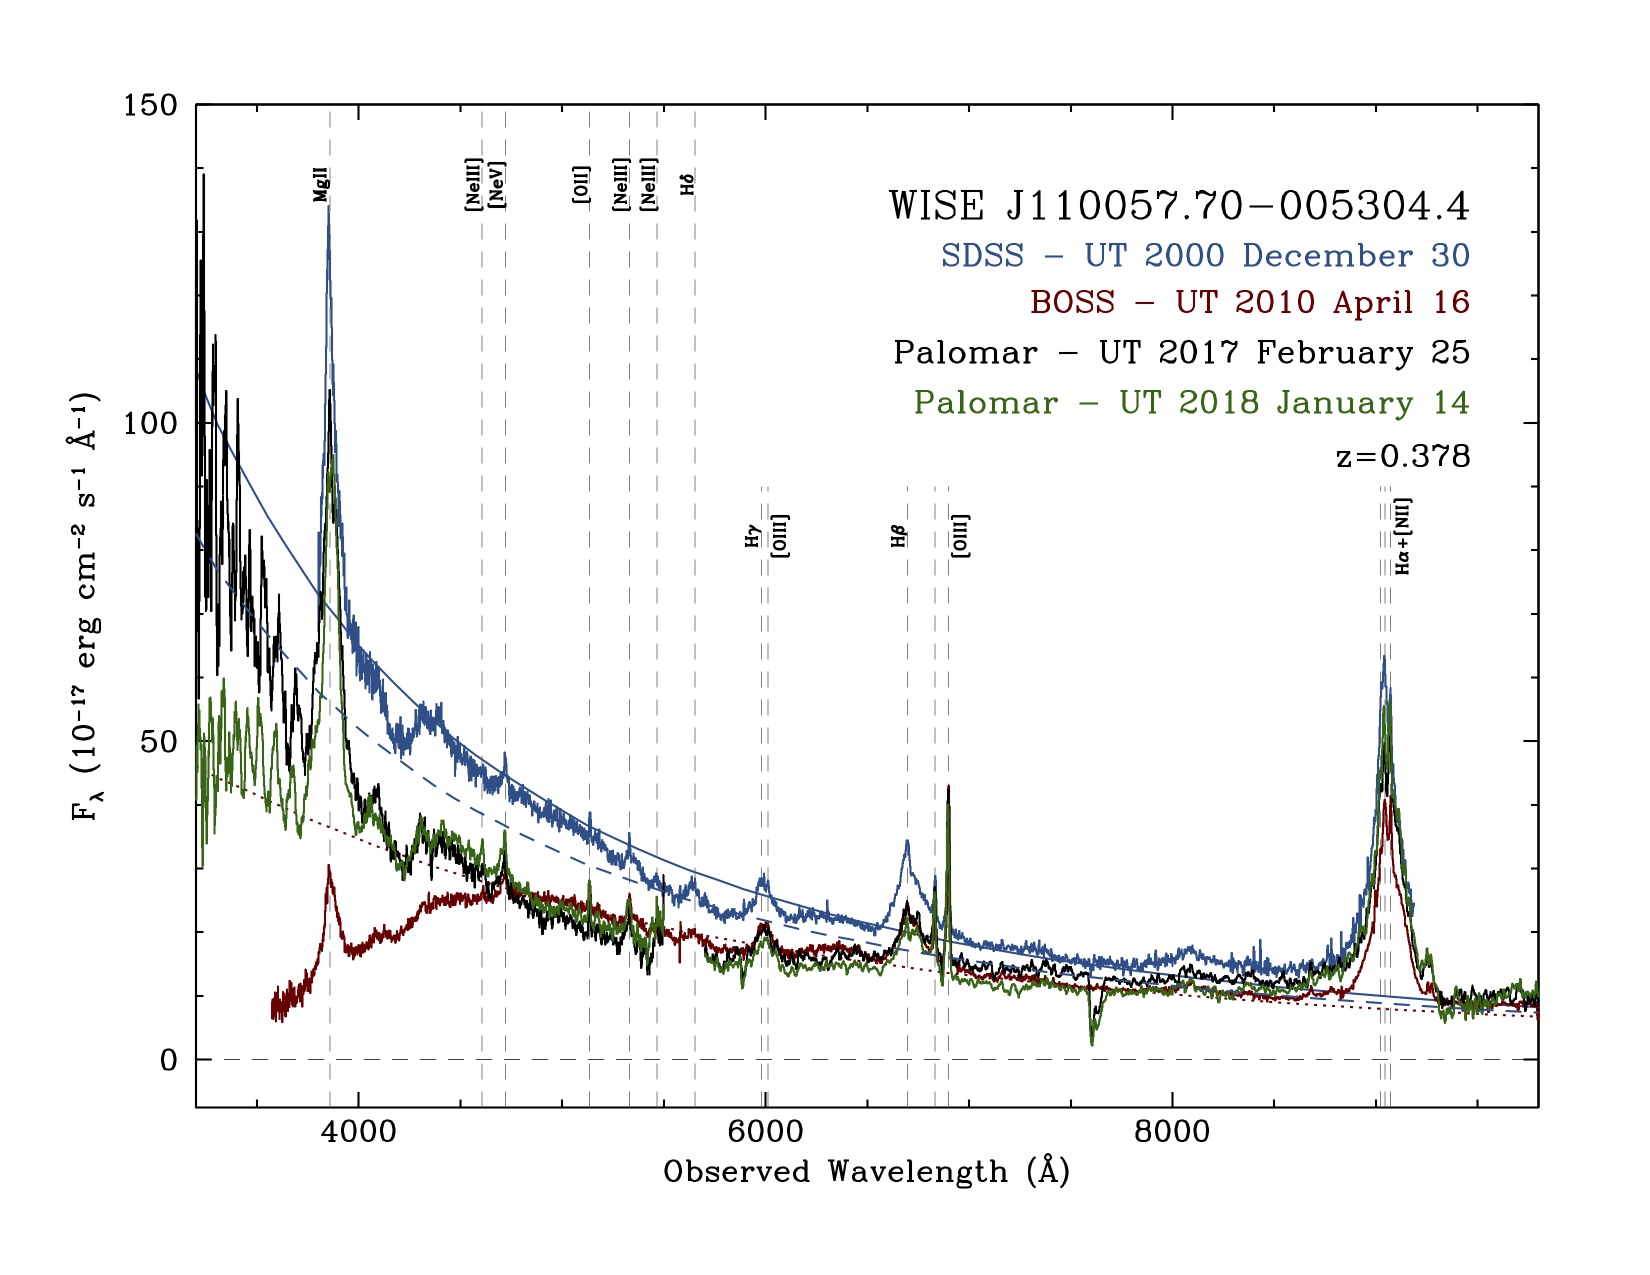
\includegraphics[width=17.00cm, height=14.00cm, trim=0.0cm 0.0cm 0.0cm 0.0cm, clip]
  {../plots/spectra/w1100m0053_sdss_palomar2.jpg}
  \caption[]{Optical spectra of J1100-0053 obtained on MJD 51908
(blue; SDSS), 55302 (red; BOSS), 57809 (black; Palomar) and 58132
(green; Palomar). Spectra have been renormalized to maintain a
constant \oiii luminosity. Over the past two decades, the UV continuum
and broad lines have changed significantly for this quasar.  In
particular, the 2nd-epoch BOSS spectrum from 2010 shows the rare
occurrence of a temporary collapse of the UV continuum.  Smooth lines
show three simple thermal accretion disk models of the continuum.  The
solid blue line shows an inflated disk with non-zero torque at the
ISCO \cite[e.g.,][]{Sirko_Goodman2003}, while the dashed blue line
shows the same model, but with zero torque at the ISCO \cite[i.e.,
equivalent to a simple $\alpha$-disk model,][]{SS73}.  Torque at the
ISCO, possibly due to magnetic fields threading the inner disk and
plunging region, heats the inner disk, causing it to puff up and
become more UV luminous.  The dotted red line shows a modified
zero-torque model where the thermal disk emission interior to $80
r_{\rm g}$ is suppressed by a factor of 10.}
  \label{fig:J110057_spectra}
\end{figure}
%%%%%%%%%%%%%%%%%%%%%%%%%%%%%%%%%%%%%%%%%%%%%%%%%%%%%%%%%%%%% 
%%%%%%%%%%%%%%%%%%%%%%%%%%%%%%%%%%%%%%%%%%%%%%%%%%%%%%%%%%%%% 
%%
%%
%%     SECTION 2   SECTION 2   SECTION 2   SECTION 2   SECTION 2   SECTION 2  
%%     SECTION 2   SECTION 2   SECTION 2   SECTION 2   SECTION 2   SECTION 2  
%%     SECTION 2   SECTION 2   SECTION 2   SECTION 2   SECTION 2   SECTION 2  
%%
%%
%%%%%%%%%%%%%%%%%%%%%%%%%%%%%%%%%%%%%%%%%%%%%%%%%%%%%%%%%%%%%
%%%%%%%%%%%%%%%%%%%%%%%%%%%%%%%%%%%%%%%%%%%%%%%%%%%%%%%%%%%%%
\section{Target Selection and Observations}  
We started by matching the SDSS-III Baryon Oscillation Spectroscopic
Survey (BOSS) Data Release 12 Quasar catalog \cite[DR12Q;
][]{Paris2017} to the NEOWISE-R IR data (WISE W1 at 3.4$\mu$m, WISE W2
at 4.6$\mu$m). We found $\approx$200 objects identified by a factor of 2
or more change in the observed WISE W1 and W2 bands over the course of
typically three or four years \citep[see][and the Supplemental
Material for the detailed NEOWISE-R selection]{Meisner2017b}. Visually
inspecting these 200 objects, we examined the change in optical colour
using the SDSS and DECaLS imaging surveys in order to identify
changing-look quasar candidates.  From this inspection, a list of
$\approx$70 priority targets was derived, and with spectra already
from SDSS and BOSS, J1100-0053 was an early target. We obtained a
third and fourth epoch of optical spectroscopy from the Palomar 5m
telescope.

Figure~\ref{fig:J110057_LC_CRTS} presents the light curve of
J1100-0053.  Along with WISE IR data, optical data from the SDSS,
Catalina Real-time Transient Survey \citep[CRTS;][]{Drake2009,
Mahabal2011}, the Lincoln Near-Earth Asteroid Research \citep[LINEAR;
][]{Sesar2011} program and the Panoramic Survey Telescope and Rapid
Response System \citep[PanSTARRS;][]{Kaiser2010, Stubbs2010,
Tonry2012, Magnier2013} are
available. Figure~\ref{fig:J110057_spectra} shows the four optical
spectra of J1100-0053 from SDSS, BOSS and Palomar observations.  The
first-epoch SDSS spectrum shows a typical blue quasar, but the blue
continuum decreases by nearly a factor or ten in flux in the second
epoch BOSS spectrum taken 10 years later. The blue continuum then
returns in the third epoch spectrum taken another 7 years later,
albeit at a diminished level relative to the initial spectrum. The
fourth epoch spectrum is very similar to the third epoch.  The
Supplemental Material gives further observational details.

While continuum changes in the rest-frame UV/optical spectra of
quasars are not a new discovery (see e.g., \cite{Clavel1991}, the
review by \cite{Ulrich1997} and more recent studies by
\cite{VandenBerk2004, Pereyra2006, MacLeod2010, Guo2016b}), the
identification of a ``UV collapse'' has only recently been noted by
\cite{Guo2016}.  Those authors report the first discovery of a UV
cutoff quasar, SDSS J231742.60 +000535.1 (hereafter J2317+0005;
redshift $z = 0.32$), observed by SDSS three times, on 2000 September
29, 2001 September 25, and 2001 October 18. In the case of J2317+0005,
a cycle of UV emission collapse, quasar dimming, and recovery was
observed over the course of just a few weeks. For J1100-0053, the
cycle is far longer; however the combination of optical and infrared
light curves, as well as observing J1100-0053 at four separate
spectral stages is currently unique. As such, J1100-0053 and
J2317+0005 are now two archetypal objects that any accretion disk
model must predict and explain \cite{Lawrence2018}.


%%%%%%%%%%%%%%%%%%%%%%%%%%%%%%%%%%%%%%%%%%%%%%%%%%%%%%%%%%%%%
%%%%%%%%%%%%%%%%%%%%%%%%%%%%%%%%%%%%%%%%%%%%%%%%%%%%%%%%%%%%%
%%
%%   SECTION 3   SECTION 3   SECTION 3   SECTION 3   SECTION 3   SECTION 3  
%%   SECTION 3   SECTION 3   SECTION 3   SECTION 3   SECTION 3   SECTION 3  
%%   SECTION 3   SECTION 3   SECTION 3   SECTION 3   SECTION 3   SECTION 3  
%%
%%%%%%%%%%%%%%%%%%%%%%%%%%%%%%%%%%%%%%%%%%%%%%%%%%%%%%%%%%%%%
%%%%%%%%%%%%%%%%%%%%%%%%%%%%%%%%%%%%%%%%%%%%%%%%%%%%%%%%%%%%%
\begin{figure*}
  %% trim=l b r t 
  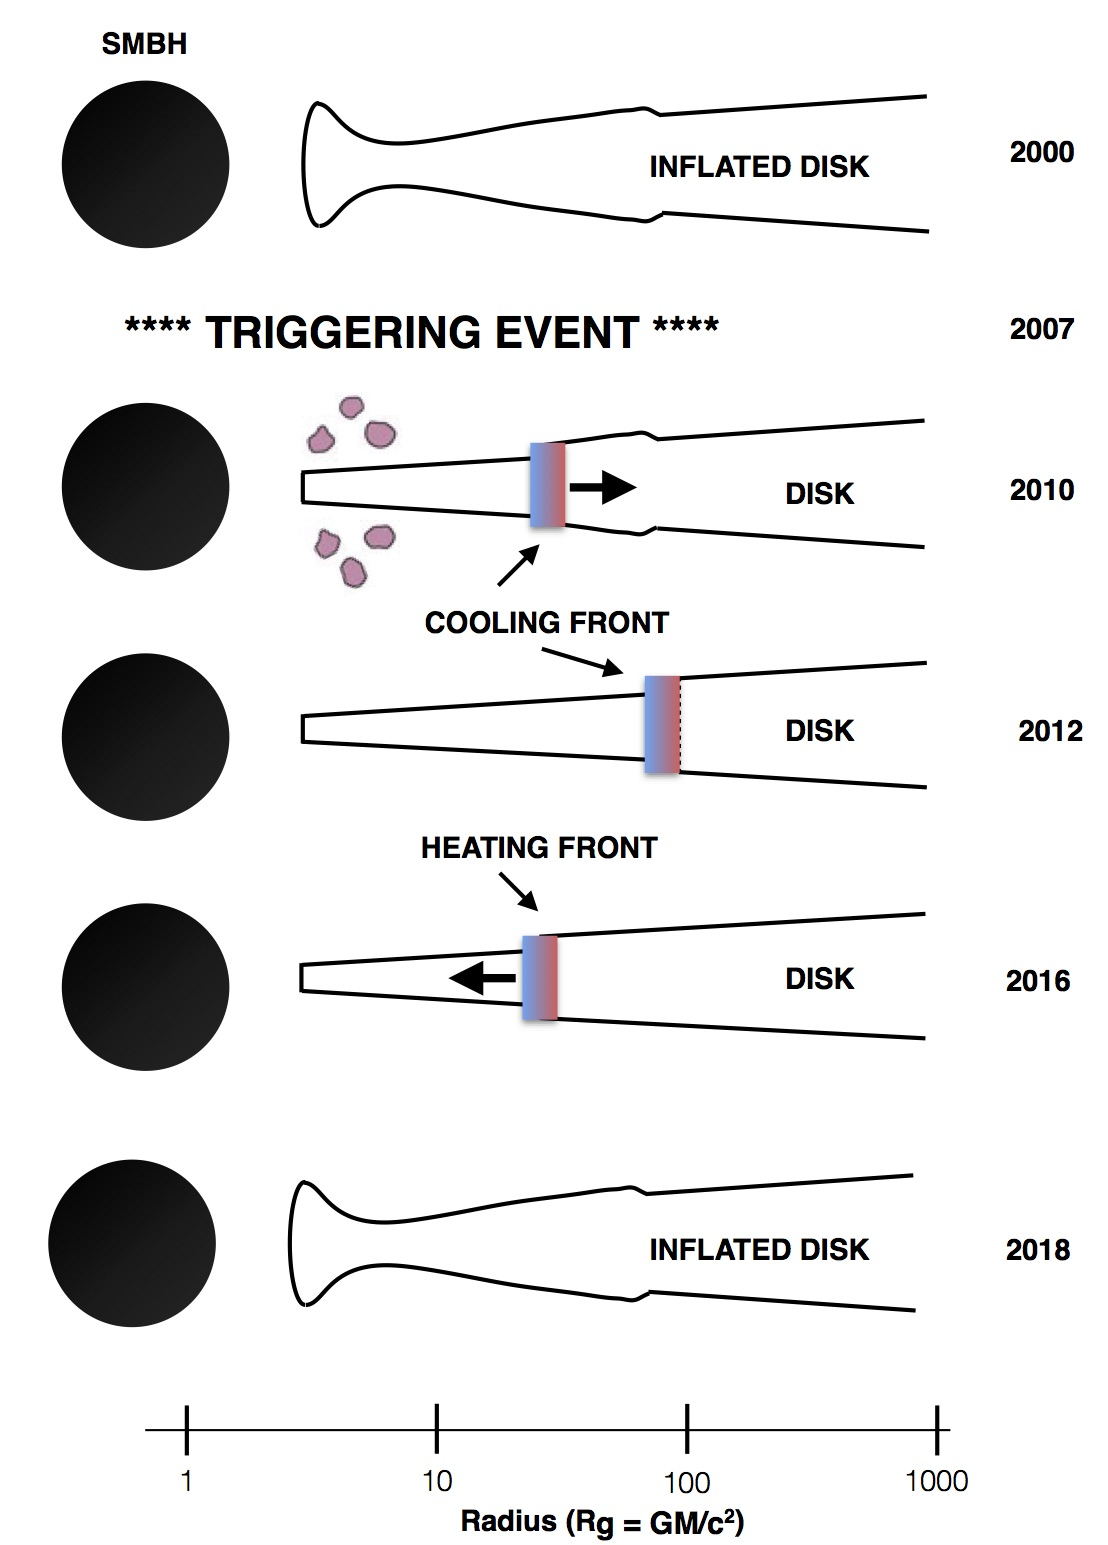
\includegraphics[width=15.4cm, height=18.75cm, trim=0.0cm 0.0cm 0.0cm 0.0cm, clip]
  {../plots/models/cartoon_v3pnt1.jpg}
  \centering
  \caption[]{
    Cartoon illustration of our model explaining the unusual spectral
evolution of J1100-0053. In 2000, corresponding to the SDSS spectral
epoch, the quasar has a standard inflated accretion disk, i.e., where
non-zero torque at the ISCO heats the inner radii of the accretion
disk, causing it to puff up \citep[e.g.,][]{Zimmerman2005}. Circa
2007, a triggering event occurs that deflates the inner disk, possibly
due to a shift in the magnetic field configuration leading to zero
torque at the ISCO.  This event leaves some scattering clouds, and
causing a cooling front to propagate outwards in the accretion disk,
traveling on the $t_{\rm front}$ time-scale 
\citep[see also][]{Hameury2009}. 
 Circa 2012, the cooling
front reaches a predicted kink in the accretion disk profile at
$\sim$100 $r_{g}$, associated with a shift in the accretion disk
opacity, e.g., Figure 2 of \cite{Sirko_Goodman2003}. A heating front
then travels radially inwards, re-heating the inner accretion disk but
on longer timescales, due to the thinner disk. We predict that in the
next year, the quasar should roughly return to its initial state.}
  \label{fig:J110057_diskmodel}
\end{figure*}

\section{Discussion} 
Our explanation for the behaviour of J1100-0053 (and J2317+0005), with a diagramatic illustration given in Figure~\ref{fig:J110057_diskmodel}, starts from the more-realistic, but $\alpha$-parameterized disk model of \cite{Sirko_Goodman2003}. In their model, the outer accretion disk is heated sufficiently to maintain stability against gravitational collapse, and small changes in temperature can lead to large changes in opacity and thus disk luminosity. In addition, the theoretical SEDs have a second peak in the near-infrared that is energetically comparable with the Big Blue Bump. \cite{Sirko_Goodman2003} assume that the viscous torque at the inner edge of their accretion disks is vanishingly small and effectively zero. This is a good assumption for very thin disks and \emph{as long as there is no connection between material inside the ISCO, i.e. the plunging region, and material at the ISCO}. 

However, if accretion disk luminosity is powered by magnetized gas losing angular momentum, it is reasonable to assume that magnetic fields are dragged across the ISCO with accreting matter, into the plunging region. As a result, we should typically expect a non-zero torque at the ISCO, as the magnetized plunging gas torques the ISCO gas. A drop in the torque at the ISCO is then most likely due to a change in $\dot{M}$ at the ISCO, which could result from a local change in $\alpha$ or a stochastic variation in the mass supply. We can regard this as the ``the triggering event''.

We then consider \cite{Zimmerman2005} who compare models with `zero' and `non-zero' torque at the ISCO, and the impact on the temperature profile of the corresponding accretion disk, when the torque changes.  In zero-torque models, temperature $T_{\rm ZT}$ goes to zero at the inner edge of the disk (since the torque vanishes there) whereas a non-zero torque temperature profile, $T_{\rm NZT}$ reaches its maximum value at the inner edge of the disk (where the torque is maximal).  Given a multi-temperature blackbody (MTB) model for disk emission, these differences at small $r_{\rm g}$ translate to large differences in the SED.  A non-zero torque at the ISCO implies that matter in the plunging region is connected (however weakly) to matter outside the ISCO, probably by magnetic fields \cite[e.g., ][]{Gammie1999, Agol_Krolik2000}. A non-zero torque at the ISCO maintains a hotter innermost disk than a condition of zero torque at the ISCO, and an assumption of non-zero torque is particularly appropriate if disk viscosity and accretion are driven by magnetic fields. Our model of thermal emission from a MTB implies changes in the region from the ISCO to $\sim$few tens-100 $r_{\rm g}$ are required to suppress flux into the observed $g$-band. In particular, we suggest a physical collapse of the disk scale height due to a cooling front propagating outward from the ISCO. The radiation properties of accretion disk with a NZTs at their inner edge was also explored by \cite{Cao2003} and \cite{Cannizzo1998b} describe in detail, the change at the ISCO is physically related to this thermal front. 

We note that \cite{Hameury2009} investigate thermal-viscous instabilities in AGN, and find that a physical mechanism of propogating cooling and heating fronts is found, and that these fronts propagate on much shorter time scales than the viscous time.  The model in \cite{Hameury2009} makes a firm prediction of this back and forth propagation of cooling and heating fronts on a short time scale, while noting that the surface density at smaller radii does not change so quickly and hence $\dot{M}$ fluctuates on a longer timescale. 

For J1100-0053 we start with an inflated slim disk and apply our model as follows. We assume a non-zero torque at the ISCO and $h/r\sim0.2$ (where $h$ and $r$ are the scale-height and radius of the accretion disk, respectively) inside of $r\sim100 r_{\rm g}$. This is the initial state circa 2000 (MJD 51900). In order to explain data subsequent to 2007, we assume a cooling front propagates out from the ISCO over a timescale $t_{\rm front}$. The front propagation timescale is $ t_{\rm front} \sim 10 \; {\rm years} \left(\frac{h/r}{0.05}\right)^{-1} \left(\frac{\alpha}{0.3}\right)^{-1} \left(\frac{r}{225r_{g}}\right)^{3/2} \frac{r_{g}}{c}$, and $\alpha$ is the traditional kinematic viscosity. As noted above, one simple, plausible trigger for this cooling front is that the non-zero torque condition at theISCO changes to a (more nearly) zero-torque condition. This dramatic decrease in the torque at the ISCO leads to a drastically cooler, thinner innermost disk. As the cooling front propagates, the drop in temperature leads to a drop in flux. To fit the observed spectra, our model has the cooler regions behind the front emitting 10\% the flux of the initial hotter disk, and assumes the disk height drops by a factor $\sim$2. The dimming of the inner disk causes a drop in the ionizing photon flux, which will cause the Balmer lines to drop in flux after a light travel time of months and the IR emission from the outer disk/torus to drop in flux after a light travel time of $\sim$3 years \citep{Sirko_Goodman2003, Koshida2014, Jun2015}.

If the inner accretion disk is usually inflated \cite[see e.g., ][]{Sirko_Goodman2003, Thompson2005, Hopkins_Quataert2011}, such a cooling front will naturally produce a collapse in the disk scale height, triggering a decrease in flux moving from UV to longer optical wavelengths, and a temporarily thicker scattering atmosphere, further decreasing flux at short wavelengths (see Fig.~\ref{fig:J110057_diskmodel}).  Given our disk parameters, outward front propagation timescales are months-to-years, corresponding with observed timescales for optical emission moving from shorter to longer wavelengths as the radius of the cooling front increases. A decrease in the UV flux would be expected to cause a decrease in IR flux, as the heating of the IR-emitting dusty torus is reduced; however, there should be a delay due to light travel time \cite[e.g., ][]{Jun2015}. By 2010 (MJD 55300) the front has reached $r\sim50 r_{g}$. During that time, the collapsing disk height increases the number density of scatterers and the temporary cold phase formed at the disk surface produces the remarkable blue downturn in the 2010 spectrum. The cooling front continues to propagate radially outward but cools less efficiently at larger disk radii. 

Eventually, very much in the same vein as discussed by \cite{Hameury2009}, somewhere in the disk, $\Sigma$ reaches the critical surface density $\Sigma_{\rm max}$, and that triggers the heating instability. A heating front propagates back inwards, analagous to the well-known accretion disk limit cycle mechanism in models of dwarf novae outbursts \cite[e.g.,][]{Cannizzo1998}. The returning heating front travels more slowly because the disk is thinner (and $t_{\rm front}$ is inversely proportional to $h/r$) and will re-inflate the disk as it propagates inwards towards the SMBH. This means the return to normal will be asymmetric in time, as observed, and the shortest wavelength bands bottom out first, because that wavelength is dominated by emission coming from $r\sim100r_{g}$ (see also discussion in the Supplemental Material).

Using \cite{Ford2018} and \cite{Sirko_Goodman2003}, Figure~\ref{fig:J110057_diskmodel} shows a model for a $M_{\rm BH}=7\times 10^{8} M_{\odot}$, with an accretion rate in units of Eddington accretion, $\dot{M}=0.070$ (appropriate for J1100-0053), radiative efficiency of $\epsilon=0.1$ inner disk radius of $6r_{\rm g}$ and outer disk radius of $10,000 r_{g}$. The resulting model spectra can be seen in Figure~\ref{fig:J110057_spectra}. We expect the front to return to the ISCO in mid-to-late 2018. That means the broad Balmer lines will come back a few months later, but the WISE IR flux should return to full flux in 2021. We note the IR brightness of J2317+0005 was only observed at one epoch and the change in the UV for J2317+0005 was rapid, decreasing by a factor of 3.5 at 3000\AA\ over only 23 days. This indicates that the cooling event was very brief, and given the extremal but plausible values of $h/r = 0.2-0.3$ and $r=20-25$ with $\alpha$ held at 0.3, is consistent with our model.



%%%%%%%%%%%%%%%%%%%%%%%%%%%%%%%%%%%%%%%%%%%%%%%%%%%%%%%%%%%%%%%%%%%%%%%%%%%%%%%%%
%%%%%%%%%%%%%%%%%%%%%%%%%%%%%%%%%%%%%%%%%%%%%%%%%%%%%%%%%%%%%%%%%%%%%%%%%%%%%%%%%
%%
%%
%%   SECTION 4   SECTION 4   SECTION 4   SECTION 4   SECTION 4   SECTION 4  
%%   SECTION 4   SECTION 4   SECTION 4   SECTION 4   SECTION 4   SECTION 4  
%%   SECTION 4   SECTION 4   SECTION 4   SECTION 4   SECTION 4   SECTION 4  
%%
%%
%%%%%%%%%%%%%%%%%%%%%%%%%%%%%%%%%%%%%%%%%%%%%%%%%%%%%%%%%%%%%%%%%%%%%%%%%%%%%%%%%%
%%%%%%%%%%%%%%%%%%%%%%%%%%%%%%%%%%%%%%%%%%%%%%%%%%%%%%%%%%%%%%%%%%%%%%%%%%%%%%%%%%
\section{Conclusions} 
In conclusion, by monitoring changing look quasars we introduce new
tests of models of accretion disk physics. We have shown that a simple
phenomenological model with a propagating cooling front is capable of
describing the gross spectral and temporal variations in a changing
looking quasar. Our model makes a prediction for this source, testable
over the next few years and, if confirmed, implies that changing
looking quasars as a class are driven by changes near the ISCO, close
to the SMBH. The discovery of J1100-0053 (and J2317+0005) are specific
key examples of time-domain astronomy and the resulting astrophysics
to be studied. However, even with the coverage from WISE, PanSTARRS,
SDSS, DECaLS and CRTS, we have a relatively sparse dataset which
cannot tightly constrain our theoretical model. The Zwicky Transient
Facility \citep[ZTF; ][]{Bellm2014} has very recently started and will
open a new data space with high cadence, multi-band photometric
monitoring. Along with ZTF in the very near future, the Large Synoptic
Survey Telescope \citep{Ivezic2008, LSST_ScienceBookV2} will allow
identification of the types of events such as J1100-0053 and
J2317+0005 \emph{while they are occurring}, allowing spectroscopic
monitoring. We will be able to see how long a UV collapse lasts and
closely follow its evolution.  Such data will stringently test models
of AGN disks at much higher fidelity than we are able to do with
current `Changing-Look' quasar samples.

{\bf Author Contributions.}   
N.P.R. led the project, identified J1100-0053 as interesting, obtained and conglomerated the data, developed and wrote the manuscript and co-ordinated the team.
K.E.S.F. and B.K. orginated and developed the theoretical interpretation. 
M.G. and D.S. were heavily responsible for the initial discussions and observations that were the genesis of
this project, as well as being fully involved in preparing the manuscript. 
A.M.M. produced the initial infrared variable quasar catalogs, while DL provided the optical+infra image analysis. 
D.S., M.G. and A.J.D. were part of the Palomar observing team.
N.P.R., A.M.M. and A.D. are part of the DECaLS Legacy Survey. 
H.D.J. provided the Balmer line fits and contributed to the manuscript.
R.A. and A.D. significantly contributed to the manuscript.
\smallskip
\smallskip



{\bf Availability of Data and computer analysis codes}. 
All materials, data, code and analysis algorithms are fully 
available at: 
\href{https://github.com/d80b2t/WISE\_LCs}{\tt https://github.com/d80b2t/WISE\_LCs}


\smallskip
\smallskip




%%%%%%%%%%%%%%%%%%%%%%%%%%%%%%%%%%%%%%%%%%%%%%%%%%%%%%%%%%%%%
%%%%%%%%%%%%%%%%%%%%%%%%%%%%%%%%%%%%%%%%%%%%%%%%%%%%%%%%%%%%%
%%
%%   SECTION 4   SECTION 4   SECTION 4   SECTION 4   SECTION 4   SECTION 4  
%%   SECTION 4   SECTION 4   SECTION 4   SECTION 4   SECTION 4   SECTION 4  
%%   SECTION 4   SECTION 4   SECTION 4   SECTION 4   SECTION 4   SECTION 4  
%%
%%%%%%%%%%%%%%%%%%%%%%%%%%%%%%%%%%%%%%%%%%%%%%%%%%%%%%%%%%%%%
%%%%%%%%%%%%%%%%%%%%%%%%%%%%%%%%%%%%%%%%%%%%%%%%%%%%%%%%%%%%%
%\section{Method}

%\bibliographystyle{naturemag}
\bibliography{/cos_pc19a_npr/LaTeX/tester_mnras}


\iffalse
\begin{thebibliography}{10}
\expandafter\ifx\csname url\endcsname\relax
  \def\url#1{\texttt{#1}}\fi
\expandafter\ifx\csname urlprefix\endcsname\relax\def\urlprefix{URL }\fi
\providecommand{\bibinfo}[2]{#2}
\providecommand{\eprint}[2][]{\url{#2}}

\bibitem{LaMassa2015}
\bibinfo{author}{{LaMassa}, S.~M.} \emph{et~al.}
\newblock \bibinfo{title}{{The Discovery of the First ``Changing Look'' Quasar:
  New Insights Into the Physics and Phenomenology of Active Galactic Nucleus}}.
\newblock \emph{\bibinfo{journal}{\apj}} \textbf{\bibinfo{volume}{800}},
  \bibinfo{pages}{144} (\bibinfo{year}{2015}).
\newblock \eprint{1412.2136}.

\bibitem{Runnoe2016}
\bibinfo{author}{{Runnoe}, J.~C.} \emph{et~al.}
\newblock \bibinfo{title}{{Now you see it, now you don't: the disappearing
  central engine of the quasar J1011+5442}}.
\newblock \emph{\bibinfo{journal}{\mnras}} \textbf{\bibinfo{volume}{455}},
  \bibinfo{pages}{1691--1701} (\bibinfo{year}{2016}).
\newblock \eprint{1509.03640}.

\bibitem{MacLeod2016}
\bibinfo{author}{{MacLeod}, C.~L.} \emph{et~al.}
\newblock \bibinfo{title}{{A systematic search for changing-look quasars in
  SDSS}}.
\newblock \emph{\bibinfo{journal}{\mnras}} \textbf{\bibinfo{volume}{457}},
  \bibinfo{pages}{389--404} (\bibinfo{year}{2016}).
\newblock \eprint{1509.08393}.

\bibitem{Ruan2016}
\bibinfo{author}{{Ruan}, J.~J.} \emph{et~al.}
\newblock \bibinfo{title}{{Toward an Understanding of Changing-look Quasars: An
  Archival Spectroscopic Search in SDSS}}.
\newblock \emph{\bibinfo{journal}{\apj}} \textbf{\bibinfo{volume}{826}},
  \bibinfo{pages}{188} (\bibinfo{year}{2016}).
\newblock \eprint{1509.03634}.

\bibitem{Yang2017}
\bibinfo{author}{{Yang}, Q.} \emph{et~al.}
\newblock \bibinfo{title}{{Discovery of 21 New Changing-look AGNs in Northern
  Sky}}.
\newblock \emph{\bibinfo{journal}{ArXiv e-prints}}  (\bibinfo{year}{2017}).
\newblock \eprint{1711.08122v1}.

\bibitem{Hutsemekers2017}
\bibinfo{author}{{Hutsem{\'e}kers}, D.}, \bibinfo{author}{{Ag{\'{\i}}s
  Gonz{\'a}lez}, B.}, \bibinfo{author}{{Sluse}, D.}, \bibinfo{author}{{Ramos
  Almeida}, C.} \& \bibinfo{author}{{Acosta Pulido}, J.-A.}
\newblock \bibinfo{title}{{Polarization of the changing-look quasar
  J1011+5442}}.
\newblock \emph{\bibinfo{journal}{\aap}} \textbf{\bibinfo{volume}{604}},
  \bibinfo{pages}{L3} (\bibinfo{year}{2017}).
\newblock \eprint{1707.05540}.

\bibitem{Sheng2017}
\bibinfo{author}{{Sheng}, Z.} \emph{et~al.}
\newblock \bibinfo{title}{{Mid-infrared Variability of Changing-look AGNs}}.
\newblock \emph{\bibinfo{journal}{\apjl}} \textbf{\bibinfo{volume}{846}},
  \bibinfo{pages}{L7} (\bibinfo{year}{2017}).
\newblock \eprint{1707.02686}.

\bibitem{Gezari2017}
\bibinfo{author}{{Gezari}, S.} \emph{et~al.}
\newblock \bibinfo{title}{{iPTF Discovery of the Rapid ``Turn-on'' of a
  Luminous Quasar}}.
\newblock \emph{\bibinfo{journal}{\apj}} \textbf{\bibinfo{volume}{835}},
  \bibinfo{pages}{144} (\bibinfo{year}{2017}).
\newblock \eprint{1612.04830}.

\bibitem{Rumbaugh2017}
\bibinfo{author}{{Rumbaugh}, N.} \emph{et~al.}
\newblock \bibinfo{title}{{Extreme variability quasars from the Sloan Digital
  Sky Survey and the Dark Energy Survey}}.
\newblock \emph{\bibinfo{journal}{ArXiv e-prints}}  (\bibinfo{year}{2017}).
\newblock \eprint{1706.07875}.

\bibitem{SS73}
\bibinfo{author}{{Shakura}, N.~I.} \& \bibinfo{author}{{Sunyaev}, R.~A.}
\newblock \bibinfo{title}{{Black holes in binary systems. Observational
  appearance.}}
\newblock \emph{\bibinfo{journal}{\aap}} \textbf{\bibinfo{volume}{24}},
  \bibinfo{pages}{337} (\bibinfo{year}{1973}).

\bibitem{King2012}
\bibinfo{author}{{King}, A.}
\newblock \bibinfo{title}{{Accretion disc theory since Shakura and Sunyaev}}.
\newblock \emph{\bibinfo{journal}{\memsai}} \textbf{\bibinfo{volume}{83}},
  \bibinfo{pages}{466} (\bibinfo{year}{2012}).
\newblock \eprint{1201.2060}.

\bibitem{Lawrence2012}
\bibinfo{author}{{Lawrence}, A.}
\newblock \bibinfo{title}{{The UV peak in active galactic nuclei: a false
  continuum from blurred reflection?}}
\newblock \emph{\bibinfo{journal}{\mnras}} \textbf{\bibinfo{volume}{423}},
  \bibinfo{pages}{451--463} (\bibinfo{year}{2012}).
\newblock \eprint{1110.0854}.

\bibitem{Pooley2007}
\bibinfo{author}{{Pooley}, D.}, \bibinfo{author}{{Blackburne}, J.~A.},
  \bibinfo{author}{{Rappaport}, S.} \& \bibinfo{author}{{Schechter}, P.~L.}
\newblock \bibinfo{title}{{X-Ray and Optical Flux Ratio Anomalies in Quadruply
  Lensed Quasars. I. Zooming in on Quasar Emission Regions}}.
\newblock \emph{\bibinfo{journal}{\apj}} \textbf{\bibinfo{volume}{661}},
  \bibinfo{pages}{19--29} (\bibinfo{year}{2007}).
\newblock \eprint{astro-ph/0607655}.

\bibitem{Morgan2010}
\bibinfo{author}{{Morgan}, C.~W.}, \bibinfo{author}{{Kochanek}, C.~S.},
  \bibinfo{author}{{Morgan}, N.~D.} \& \bibinfo{author}{{Falco}, E.~E.}
\newblock \bibinfo{title}{{The Quasar Accretion Disk Size-Black Hole Mass
  Relation}}.
\newblock \emph{\bibinfo{journal}{\apj}} \textbf{\bibinfo{volume}{712}},
  \bibinfo{pages}{1129--1136} (\bibinfo{year}{2010}).
\newblock \eprint{1002.4160}.

\bibitem{Morgan2012}
\bibinfo{author}{{Morgan}, C.~W.} \emph{et~al.}
\newblock \bibinfo{title}{{Further Evidence that Quasar X-Ray Emitting Regions
  are Compact: X-Ray and Optical Microlensing in the Lensed Quasar Q
  J0158-4325}}.
\newblock \emph{\bibinfo{journal}{\apj}} \textbf{\bibinfo{volume}{756}},
  \bibinfo{pages}{52} (\bibinfo{year}{2012}).
\newblock \eprint{1205.4727}.

\bibitem{Mosquera2011}
\bibinfo{author}{{Mosquera}, A.~M.} \& \bibinfo{author}{{Kochanek}, C.~S.}
\newblock \bibinfo{title}{{The Microlensing Properties of a Sample of 87 Lensed
  Quasars}}.
\newblock \emph{\bibinfo{journal}{\apj}} \textbf{\bibinfo{volume}{738}},
  \bibinfo{pages}{96} (\bibinfo{year}{2011}).
\newblock \eprint{1104.2356}.

\bibitem{Balbus_Hawley1991}
\bibinfo{author}{{Balbus}, S.~A.} \& \bibinfo{author}{{Hawley}, J.~F.}
\newblock \bibinfo{title}{{A powerful local shear instability in weakly
  magnetized disks. I - Linear analysis. II - Nonlinear evolution}}.
\newblock \emph{\bibinfo{journal}{\apj}} \textbf{\bibinfo{volume}{376}},
  \bibinfo{pages}{214--233} (\bibinfo{year}{1991}).

\bibitem{McKernan2014}
\bibinfo{author}{{McKernan}, B.}, \bibinfo{author}{{Ford}, K.~E.~S.},
  \bibinfo{author}{{Kocsis}, B.}, \bibinfo{author}{{Lyra}, W.} \&
  \bibinfo{author}{{Winter}, L.~M.}
\newblock \bibinfo{title}{{Intermediate-mass black holes in AGN discs - II.
  Model predictions and observational constraints}}.
\newblock \emph{\bibinfo{journal}{\mnras}} \textbf{\bibinfo{volume}{441}},
  \bibinfo{pages}{900--909} (\bibinfo{year}{2014}).
\newblock \eprint{1403.6433}.

\bibitem{Mainzer2014}
\bibinfo{author}{{Mainzer}, A.} \emph{et~al.}
\newblock \bibinfo{title}{{Initial Performance of the NEOWISE Reactivation
  Mission}}.
\newblock \emph{\bibinfo{journal}{\apj}} \textbf{\bibinfo{volume}{792}},
  \bibinfo{pages}{30} (\bibinfo{year}{2014}).
\newblock \eprint{1406.6025}.

\bibitem{Meisner2017a}
\bibinfo{author}{{Meisner}, A.~M.}, \bibinfo{author}{{Lang}, D.} \&
  \bibinfo{author}{{Schlegel}, D.~J.}
\newblock \bibinfo{title}{{Deep Full-sky Coadds from Three Years of WISE and
  NEOWISE Observations}}.
\newblock \emph{\bibinfo{journal}{\aj}} \textbf{\bibinfo{volume}{154}},
  \bibinfo{pages}{161} (\bibinfo{year}{2017}).
\newblock \eprint{1705.06746}.

\bibitem{Meisner2017b}
\bibinfo{author}{{Meisner}, A.~M.} \emph{et~al.}
\newblock \bibinfo{title}{{Searching for Planet Nine with Coadded WISE and
  NEOWISE-Reactivation Images}}.
\newblock \emph{\bibinfo{journal}{\aj}} \textbf{\bibinfo{volume}{153}},
  \bibinfo{pages}{65} (\bibinfo{year}{2017}).
\newblock \eprint{1611.00015}.

\bibitem{Assef2017}
\bibinfo{author}{{Assef}, R.~J.} \emph{et~al.}
\newblock \bibinfo{title}{{The WISE AGN Catalog}}.
\newblock \emph{\bibinfo{journal}{1706.09901v1}}  (\bibinfo{year}{2017}).
\newblock \eprint{1706.09901}.

\bibitem{Paris2017}
\bibinfo{author}{{P{\^a}ris}, I.}, \bibinfo{author}{{Petitjean}, P.},
  \bibinfo{author}{{Ross}, N.~P.} \emph{et~al.}
\newblock \bibinfo{title}{{The Sloan Digital Sky Survey Quasar Catalog: Twelfth
  data release}}.
\newblock \emph{\bibinfo{journal}{\aap}} \textbf{\bibinfo{volume}{597}},
  \bibinfo{pages}{A79} (\bibinfo{year}{2017}).
\newblock \eprint{1608.06483}.

\bibitem{Drake2009}
\bibinfo{author}{{Drake}, A.~J.} \emph{et~al.}
\newblock \bibinfo{title}{{First Results from the Catalina Real-Time Transient
  Survey}}.
\newblock \emph{\bibinfo{journal}{\apj}} \textbf{\bibinfo{volume}{696}},
  \bibinfo{pages}{870--884} (\bibinfo{year}{2009}).
\newblock \eprint{0809.1394}.

\bibitem{Mahabal2011}
\bibinfo{author}{{Mahabal}, A.~A.} \emph{et~al.}
\newblock \bibinfo{title}{{Discovery, classification, and scientific
  exploration of transient events from the Catalina Real-time Transient
  Survey}}.
\newblock \emph{\bibinfo{journal}{Bulletin of the Astronomical Society of
  India}} \textbf{\bibinfo{volume}{39}}, \bibinfo{pages}{387--408}
  (\bibinfo{year}{2011}).
\newblock \eprint{1111.0313}.

\bibitem{Sesar2011}
\bibinfo{author}{{Sesar}, B.} \emph{et~al.}
\newblock \bibinfo{title}{{Exploring the Variable Sky with LINEAR. I.
  Photometric Recalibration with the Sloan Digital Sky Survey}}.
\newblock \emph{\bibinfo{journal}{\aj}} \textbf{\bibinfo{volume}{142}},
  \bibinfo{pages}{190} (\bibinfo{year}{2011}).
\newblock \eprint{1109.5227}.

\bibitem{Kaiser2010}
\bibinfo{author}{{Kaiser}, N.} \emph{et~al.}
\newblock \bibinfo{title}{{The Pan-STARRS wide-field optical/NIR imaging
  survey}}.
\newblock In \emph{\bibinfo{booktitle}{Society of Photo-Optical Instrumentation
  Engineers (SPIE) Conference Series}}, vol. \bibinfo{volume}{7733} of
  \emph{\bibinfo{series}{Society of Photo-Optical Instrumentation Engineers
  (SPIE) Conference Series}}, \bibinfo{pages}{0} (\bibinfo{year}{2010}).

\bibitem{Stubbs2010}
\bibinfo{author}{{Stubbs}, C.~W.} \emph{et~al.}
\newblock \bibinfo{title}{{Precise Throughput Determination of the PanSTARRS
  Telescope and the Gigapixel Imager Using a Calibrated Silicon Photodiode and
  a Tunable Laser: Initial Results}}.
\newblock \emph{\bibinfo{journal}{\apjs}} \textbf{\bibinfo{volume}{191}},
  \bibinfo{pages}{376--388} (\bibinfo{year}{2010}).
\newblock \eprint{1003.3465}.

\bibitem{Tonry2012}
\bibinfo{author}{{Tonry}, J.~L.} \emph{et~al.}
\newblock \bibinfo{title}{{The Pan-STARRS1 Photometric System}}.
\newblock \emph{\bibinfo{journal}{\apj}} \textbf{\bibinfo{volume}{750}},
  \bibinfo{pages}{99} (\bibinfo{year}{2012}).
\newblock \eprint{1203.0297}.

\bibitem{Magnier2013}
\bibinfo{author}{{Magnier}, E.~A.} \emph{et~al.}
\newblock \bibinfo{title}{{The Pan-STARRS 1 Photometric Reference Ladder,
  Release 12.01}}.
\newblock \emph{\bibinfo{journal}{\apjs}} \textbf{\bibinfo{volume}{205}},
  \bibinfo{pages}{20} (\bibinfo{year}{2013}).
\newblock \eprint{1303.3634}.

\bibitem{Gammie1999}
\bibinfo{author}{{Gammie}, C.~F.}
\newblock \bibinfo{title}{{Efficiency of Magnetized Thin Accretion Disks in the
  Kerr Metric}}.
\newblock \emph{\bibinfo{journal}{\apjl}} \textbf{\bibinfo{volume}{522}},
  \bibinfo{pages}{L57--L60} (\bibinfo{year}{1999}).
\newblock \eprint{astro-ph/9906223}.

\bibitem{Agol_Krolik2000}
\bibinfo{author}{{Agol}, E.} \& \bibinfo{author}{{Krolik}, J.~H.}
\newblock \bibinfo{title}{{Magnetic Stress at the Marginally Stable Orbit:
  Altered Disk Structure, Radiation, and Black Hole Spin Evolution}}.
\newblock \emph{\bibinfo{journal}{\apj}} \textbf{\bibinfo{volume}{528}},
  \bibinfo{pages}{161--170} (\bibinfo{year}{2000}).
\newblock \eprint{astro-ph/9908049}.

\bibitem{Sirko_Goodman2003}
\bibinfo{author}{{Sirko}, E.} \& \bibinfo{author}{{Goodman}, J.}
\newblock \bibinfo{title}{{Spectral energy distributions of marginally
  self-gravitating quasi-stellar object discs}}.
\newblock \emph{\bibinfo{journal}{\mnras}} \textbf{\bibinfo{volume}{341}},
  \bibinfo{pages}{501--508} (\bibinfo{year}{2003}).
\newblock \eprint{astro-ph/0209469}.

\bibitem{Thompson2005}
\bibinfo{author}{{Thompson}, T.~A.}, \bibinfo{author}{{Quataert}, E.} \&
  \bibinfo{author}{{Murray}, N.}
\newblock \bibinfo{title}{{Radiation Pressure-supported Starburst Disks and
  Active Galactic Nucleus Fueling}}.
\newblock \emph{\bibinfo{journal}{\apj}} \textbf{\bibinfo{volume}{630}},
  \bibinfo{pages}{167--185} (\bibinfo{year}{2005}).
\newblock \eprint{astro-ph/0503027}.

\bibitem{Hopkins_Quataert2011}
\bibinfo{author}{{Hopkins}, P.~F.} \& \bibinfo{author}{{Quataert}, E.}
\newblock \bibinfo{title}{{An analytic model of angular momentum transport by
  gravitational torques: from galaxies to massive black holes}}.
\newblock \emph{\bibinfo{journal}{\mnras}} \textbf{\bibinfo{volume}{415}},
  \bibinfo{pages}{1027--1050} (\bibinfo{year}{2011}).
\newblock \eprint{1007.2647}.

\bibitem{Jun2015}
\bibinfo{author}{{Jun}, H.~D.} \emph{et~al.}
\newblock \bibinfo{title}{{Infrared Time Lags for the Periodic Quasar PG
  1302-102}}.
\newblock \emph{\bibinfo{journal}{\apjl}} \textbf{\bibinfo{volume}{814}},
  \bibinfo{pages}{L12} (\bibinfo{year}{2015}).
\newblock \eprint{1511.01515}.

\bibitem{Cannizzo1998}
\bibinfo{author}{{Cannizzo}, J.~K.}
\newblock \bibinfo{title}{{On the M$_{V}$(peak) versus Orbital Period Relation
  for Dwarf Nova Outbursts}}.
\newblock \emph{\bibinfo{journal}{\apj}} \textbf{\bibinfo{volume}{493}},
  \bibinfo{pages}{426--430} (\bibinfo{year}{1998}).
\newblock \eprint{astro-ph/9712210}.

\bibitem{Ford2018}
\bibinfo{author}{{Ford}, K.~E.~S.} \emph{et~al.}
\newblock \emph{\bibinfo{journal}{in prep.}}  (\bibinfo{year}{2018}).

\bibitem{Guo2016}
\bibinfo{author}{{Guo}, H.} \emph{et~al.}
\newblock \bibinfo{title}{{The Optical Variability of SDSS Quasars from
  Multi-epoch Spectroscopy. III. A Sudden UV Cutoff in Quasar SDSS
  J2317+0005}}.
\newblock \emph{\bibinfo{journal}{\apj}} \textbf{\bibinfo{volume}{826}},
  \bibinfo{pages}{186} (\bibinfo{year}{2016}).
\newblock \eprint{1605.07301}.

\end{thebibliography}

\fi


\end{document}
